\documentclass{article}
\usepackage{amsmath}
\usepackage{amssymb}
\usepackage{enumitem}
\usepackage{algorithm}
\usepackage{listings}
\usepackage{color,xcolor}
\usepackage[T1]{fontenc}
\usepackage{fontawesome}
\usepackage{etoolbox}
\usepackage{multicol}
\usepackage{geometry}
\usepackage[colorlinks=true,linkcolor=blue,urlcolor=red,bookmarksopen=true]{hyperref}
\usepackage{tikz, pgfplots, tkz-euclide,calc}
\usepackage[outline]{contour} % halo around text
    \contourlength{1.2pt}
    \usetikzlibrary{positioning,calc}
    \usetikzlibrary{backgrounds}
    \usepgfplotslibrary{fillbetween}
    \pgfplotsset{compat=1.12} 
    \colorlet{mydarkblue}{blue!30!black}
    \usetikzlibrary{patterns,snakes,shapes.arrows,3d,patterns.meta,angles,quotes}
    \geometry{
        total = {160mm, 237mm},
        left = 25mm,
        right = 35mm,
        top = 30mm,
        bottom = 30mm,
      }
\usepackage{physics}
\usepackage{ifthen}
\usepackage[outline]{contour} % glow around text
\tikzset{>=latex} % for LaTeX arrow head
\contourlength{1.2pt}
\colorlet{myred}{red!65!black}
\tikzstyle{ground}=[preaction={fill,top color=black!10,bottom color=black!5,shading angle=20},
                    fill,pattern=north east lines,draw=none,minimum width=0.3,minimum height=0.6]
\tikzstyle{mass}=[line width=0.6,red!30!black,fill=red!40!black!10,rounded corners=1,
                  top color=red!40!black!20,bottom color=red!40!black!10,shading angle=20]
\tikzstyle{mass shadow}=[line width=0.6,rounded corners=1,loosely dashed]
\tikzstyle{rope}=[brown!70!black,line width=1.2,line cap=round] %very thick

% FORCES SWITCH
\tikzstyle{force}=[->,myred,thick,line cap=round]
\tikzstyle{Fproj}=[force,myred!40]
\newcommand{\vbF}{\vb{F}}
\newboolean{showforces}
\setboolean{showforces}{true}

\usepackage{tcolorbox}
     \tcbuselibrary{listings,skins}

\newcommand{\enter}{\raisebox{-1.8pt}{
\begin{tikzpicture}[scale=0.3]
    \draw[thin,fill=lightgray] (0,0) rectangle (2,1);
    \draw (0.3,0.3) -- (0.7,0.3)--(0.7,0.6);     
\end{tikzpicture}}}

\definecolor{HIMAmuda}{HTML}{01D1FD}
\definecolor{HIMAtua}{HTML}{02016A}
\definecolor{HIMAabu}{HTML}{CBCBCC}
\definecolor{pgray}{rgb}{0.5,0.5,0.5}
\definecolor{pblue}{rgb}{0.13,0.13,1}
\definecolor{pgreen}{rgb}{0,0.5,0}
\definecolor{pred}{rgb}{0.9,0,0}
\definecolor{pgrey}{rgb}{0.46,0.45,0.48}
\definecolor{pcyan}{HTML}{D4EFFC}
\definecolor{lblue}{HTML}{00AEEF}
\definecolor{input}{HTML}{AAE1FA}
\definecolor{bg}{rgb}{0.95, 0.95, 0.92}
\definecolor{vscode}{HTML}{282A36}
\definecolor{PastelGreen}{HTML}{77DD77}

\newcommand{\inputscan}[1]{\raisebox{0pt}[1pt]{\colorbox{darkgray}{#1}}}

\usepackage{listings}

\lstdefinestyle{Liang}{
language=Java,
showspaces=false,
showtabs=false,
breaklines=true,
showstringspaces=false,
breakatwhitespace=true,
commentstyle=\color{pgray},
keywordstyle=\color{pblue},
stringstyle=\color{pgreen},
basicstyle=\small\ttfamily,
frame=single,
backgroundcolor=\color{pcyan},
escapeinside={(*}{*)},}

\lstdefinestyle{output}{
    language=Java,
    backgroundcolor=\color{vscode},
    basicstyle=\small\ttfamily\color{white},
    frame=none,
    escapeinside={(*}{*)},
    showspaces=false,
    showtabs=false,
    breaklines=true,
    showstringspaces=false,
    breakatwhitespace=true,
    keywordstyle=\color{white},
    }

\lstdefinestyle{standard}{
    language=Java,
    showspaces=false,
    showtabs=false,
    breaklines=true,
    showstringspaces=false,
    breakatwhitespace=true,
    commentstyle=\color{pgray},
    keywordstyle=\color{pblue},
    stringstyle=\color{pgreen},
    basicstyle=\small\ttfamily,
    frame=single,
    backgroundcolor=\color{bg},
    escapeinside={(*}{*)},}
\lstset{style=Liang}

\newtcblisting{RunCode}[1][enhanced,drop shadow]{
    arc=0pt, outer arc=0pt,
    boxsep=1pt,
    boxrule=2pt,
    auto outer arc,
    colback=vscode,
    colframe=bg,
    listing only, 
    listing style=output,
    title=\color{black}Ex. Output,
    #1
    }
\newtcblisting{RunCodeMore}[1][enhanced,drop shadow]{
    arc=0pt, outer arc=0pt,
    boxsep=1pt,
    boxrule=2pt,
    auto outer arc,
    colback=vscode,
    colframe=bg,
    listing only, 
    listing style=output,
    #1
    }

\newtcolorbox{hint}[1][]{
    colback=PastelGreen!5!white, 
    colframe=PastelGreen!75!black,
    fonttitle=\bfseries, 
    colbacktitle=PastelGreen!85!black,
    enhanced, 
    attach boxed title to top left={yshift=-2mm}, 
    title=Hint,
    before upper=\renewcommand\thempfootnote{\Roman{mpfootnote}},
    #1
}

\newtcolorbox{req}[1][]{
    colback=lblue!5!white, 
    colframe=lblue!75!black,
    fonttitle=\bfseries, 
    colbacktitle=lblue!85!black,
    enhanced, 
    attach boxed title to top left={yshift=-2mm}, 
    title=Input,
    before upper=\renewcommand\thempfootnote{\Roman{mpfootnote}},
    #1
}

\newtcolorbox{out}[1][]{
    colback=HIMAtua!5!white, 
    colframe=HIMAtua!75!black,
    fonttitle=\bfseries, 
    colbacktitle=HIMAtua!85!black,
    enhanced, 
    attach boxed title to top left={yshift=-2mm}, 
    title=Output,
    before upper=\renewcommand\thempfootnote{\Roman{mpfootnote}},
    #1
}

\renewcommand{\thesubsection}{\arabic{subsection}}
\newcommand{\R}{\mathbb{R}}
\newcommand{\Z}{\mathbb{Z}}
\newcommand{\N}{\mathbb{N}}
\renewcommand{\figurename}{Gambar}

\pgfmathdeclarefunction{gauss}{3}{%
  \pgfmathparse{1/(#3*sqrt(2*pi))*exp(-((#1-#2)^2)/(2*#3^2))}%
}
\pgfmathdeclarefunction{cdf}{3}{%
  \pgfmathparse{1/(1+exp(-0.07056*((#1-#2)/#3)^3 - 1.5976*(#1-#2)/#3))}%
}
\pgfmathdeclarefunction{fq}{3}{%
  \pgfmathparse{1/(sqrt(2*pi*#1))*exp(-(sqrt(#1)-#2/#3)^2/2)}%
}
\pgfmathdeclarefunction{fq0}{1}{%
  \pgfmathparse{1/(sqrt(2*pi*#1))*exp(-#1/2)}%
}

\title{\textbf{Week 6 Assigment}}
\date{21 Oktober 2024}
\author{Teosofi H.A \& Hafidz M.}

\begin{document}
    \maketitle
    \pagenumbering{gobble}

    \section*{Tugas Mandiri}
    \begin{enumerate}[label=]
        \item \textbf{(Metode Statistika)}\\
        Distribusi normal adalah distribusi probabilitas yang paling penting dalam statistika. Distribusi ini memiliki bentuk kurva lonceng dan simetris terhadap nilai rata-rata $\mu$ dan memiliki standar deviasi $\sigma$. Distribusi normal memiliki fungsi kepadatan probabilitas sebagai berikut:
        \begin{equation*}
            f(x)=\dfrac{1}{\sqrt{2\pi}\sigma}e^{-\frac{(x-\mu)^2}{2\sigma^2}},\quad -\infty<x<\infty
        \end{equation*} 
        Dalam mata kuliah Metode Statistika, kalian diajarkan untuk mengubah distribusi normal yang umum menjadi distribusi normal standar dengan cara menghitung nilai $z$-score. Konsep yang digunakan adalah subtitusi nilai $z=\dfrac{x-\mu}{\sigma}$ pada integral distribusi normal umum.\\
        \begin{figure}[h!]
          \centering
          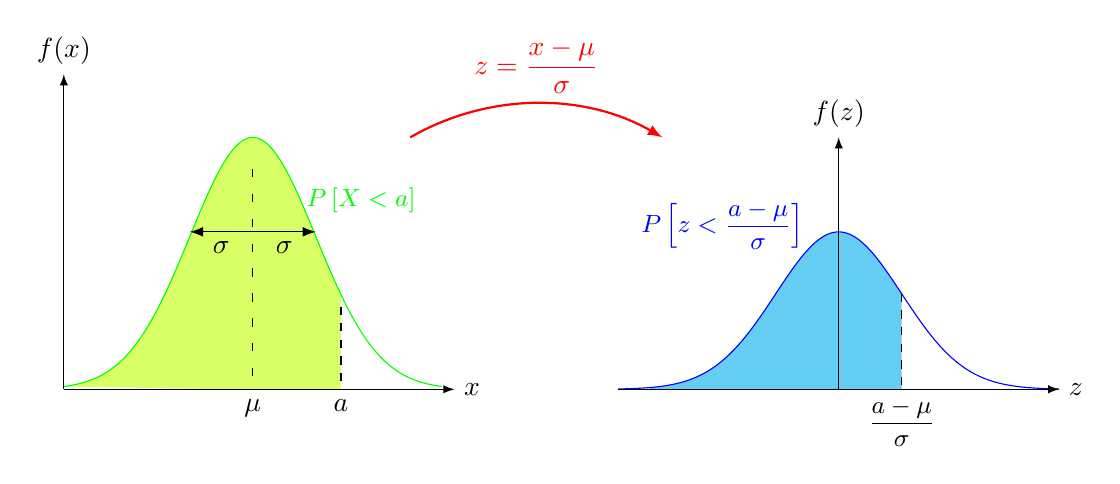
\begin{tikzpicture}[scale=0.8]
            % define normal distribution function 'normaltwo'
            \def\normaltwo{\x,{4*1/exp(((\x-3)^2)/2)}}
            
            % input y parameter
            \def\y{4.4}
            
            % this line calculates f(y)
            \def\fy{3.5*1/exp(((\y-3)^2)/2)}
            
            % Shade orange area underneath curve.
            \fill [fill=lime!60] (2.6,0) -- plot[domain=0:4.4] (\normaltwo) -- ({\y},0) -- cycle;
            
            % Draw and label normal distribution function
            \draw[color=green,domain=0:6,samples=100] plot (\normaltwo) node[right] {};
            
            % Add dashed line dropping down from normal.
            \draw[dashed] ({\y},{\fy}) -- ({\y},0) node[below] {$a$};
            
            % Optional: Add axis labels
            \draw[loosely dashed] (3,3.5)--(3,0) node[below] {$\mu$};
            \draw[-Latex] (3,2.5)--(4,2.5) node[midway,below] {$\sigma$};
            \draw[-Latex] (3,2.5)--(2,2.5) node[midway,below] {$\sigma$};
            \draw (3.7,3) node[right] {\small\color{green}$P\left[X<a\right]$};
            
            % Optional: Add axes
            \draw[->] (0,0) -- (6.2,0) node[right] {$x$};
            \draw[->] (0,0) -- (0,5) node[above] {$f(x)$};

            \draw[thick, ->,red] (5.5,4) arc (120:60:4) node[midway,above] {$z=\dfrac{x-\mu}{\sigma}$};
            
            \begin{scope}[xshift=350]
              % define normal distribution function 'normaltwo'
              \def\normaltwo{\x,{2.5*1/exp(((\x)^2)/2)}}
              
              % input y parameter
              \def\y{1}
              
              % this line calculates f(y)
              \def\fy{2.5*1/exp(((\y)^2)/2)}
              
              % Shade orange area underneath curve.
              \fill [fill=lblue!60] (-3,0) -- plot[domain=-3:1] (\normaltwo) -- ({\y},0) -- cycle;
              
              % Draw and label normal distribution function
              \draw[color=blue,domain=-3.5:3.5,samples=100] plot (\normaltwo) node[right] {};
              
              % Add dashed line dropping down from normal.
              \draw[dashed] ({\y},{\fy}) -- ({\y},0) node[below] {\small$\dfrac{a-\mu}{\sigma}$};
              
              % Optional: Add axis labels
              \draw (-.4,2.6) node[left] {\small\color{blue}$P\left[z<\dfrac{a-\mu}{\sigma}\right]$};
              
              % Optional: Add axes
              \draw[->] (-3.5,0) -- (3.5,0) node[right] {$z$};
              \draw[->] (0,0) -- (0,4) node[above] {$f(z)$};
            \end{scope}
          \end{tikzpicture}
          \caption{Distribusi Normal Umum dan Distribusi Normal Standar}
        \end{figure}

        Luasan yang diarsir pada dua kurva di atas bernilai sama yang dimana mewakili peluang kumulatif dari distribusi normal. Sebelumnya kita hanya mengethaui nilai distribusi normal berdasarkan dari tabel, namun tahukah bahwa kamu bisa menghitungnya sendiri tanpa harus melihat tabel?

        Nilai kumulatif dari distribusi normal standar dapat dihitung menggunakan integral berikut:
        \begin{equation*}
            P\left[Z<z\right]=\int_{-\infty}^{z}\dfrac{1}{\sqrt{2\pi}}e^{-\frac{t^2}{2}}dt
        \end{equation*}
        Integral diatas merupakan salah satu \textit{non-elementary integral}\footnote{Integral yang hasilnya bukan merupakan fungsi yang telah kita ketahui pada umumnya} sehingga kita tidak bisa menghitungnya secara analitik.

        Rumus aproksimasi yang digunakan untuk menghitung integral di atas dapat kita gunakan Deret Taylor\footnote{Akan dipelajari di Kalkulus 2 bab terakhir} dari fungsi distribusi normal standar. 
        \begin{equation*}
            P\left[Z<z\right]\approx\frac{1}{2}+\frac{1}{\sqrt{2\pi}}\sum^n_{k=0}\dfrac{(-1)^k\cdot z^{2k+1}}{(2k+1)\cdot k!\cdot 2^k}
        \end{equation*}
        Jika nilai $n$ semakin besar, maka hasil aproksimasi akan semakin mendekati nilai sebenarnya.\\

        Buatlah program yang dapat menghitung nilai kumulatif dari distribusi normal standar dengan menggunakan rumus aproksimasi di atas dengan mempertimbangkan nilai eror yang diberikan oleh pengguna. 

        \begin{hint}
            Buatlah \texttt{loop} untuk menghitung $\displaystyle\sum^n_{k=0}\dfrac{(-1)^k\cdot z^{2k+1}}{(2k+1)\cdot k!\cdot 2^k}$ yang akan berjalan hingga nilai eror yang diberikan oleh pengguna terpenuhi. Misalkan $\varepsilon$ adalah nilai eror yang diberikan oleh pengguna, maka program akan berhenti ketika nilai 
            \[\left|\dfrac{(-1)^n\cdot z^{2n+1}}{(2n+1)\cdot n!\cdot 2^n}\right|<\varepsilon\]
            untuk $n$ yang dimana menyatakan banyaknya iterasi pada \texttt{loop}.
        \end{hint}
        \begin{req}
          \begin{itemize}
            \item $z=:$ Posisi relatif sebuah nilai dalam distribusi normal standar\\
            $-8<z\leq 8,\quad z\in\R$
            \item $\varepsilon=:$ Nilai eror yang diberikan oleh pengguna\\
            $0<\varepsilon\leq 10^{-1},\quad \varepsilon\in\R$
        \end{itemize}
        \end{req}
        \begin{out}
            \begin{itemize}
              \item $n=:$ Banyak iterasi yang dilakukan oleh program setelah toleransi eror yang diberikan oleh pengguna terpenuhi.\\
              $n\in\N$
              \item $P\left[Z<z\right]=:$ Nilai kumulatif dari distribusi normal standar.\footnote{Bisa dibandingkan dengan nilai yang ada pada tabel distribusi normal standar}\\
              $0\leq P\left[Z<z\right]\leq 1$
            \end{itemize}
        \end{out}
        \begin{RunCode}
Masukkan nilai z: (*\inputscan{1} \enter*)
Toleransi error: (*\inputscan{10e-5} \enter*)
Diperlukan iterasi sebanyak 5
P( Z <= 1.0 ) = 0.8413441191604394
        \end{RunCode}
        \footnotetext[3]{\texttt{10e-5} dalam bahasa java berarti $10^{-5}$}
    \end{enumerate}
\end{document}